\documentclass[10pt]{article}

% %%%%%%%%%%%%%%%%%%%%%%%%%%%%%%%%%%%%%%%%%%%%%%%%%%%%%%%%%%%%%%%%%%%%%%%%%%%%%%
% %                                 PACKAGES                                   %
% %%%%%%%%%%%%%%%%%%%%%%%%%%%%%%%%%%%%%%%%%%%%%%%%%%%%%%%%%%%%%%%%%%%%%%%%%%%%%%
% Identifies input coming with an UTF-8 format
\usepackage[utf8]{inputenc}
% Uses 8-bit T1 fonts (Latin) 
\usepackage{setspace}
 \singlespacing
% Arial font.
\usepackage[scaled]{helvet}
\renewcommand\familydefault{\sfdefault}
\usepackage[T1]{fontenc}
\setlength{\parindent}{0.4cm}
% Equations
\usepackage{amsmath}
% Enum Item
\usepackage{enumitem}
% Easy Lists
\usepackage[ampersand]{easylist}
% Tables
\usepackage{booktabs}
\usepackage{longtable}
% Hyperreferences
\usepackage{hyperref}
% Images
\usepackage{graphicx}
% Set images location
\usepackage{wrapfig}
% Position for tables and images
\usepackage{float}
% Blibliography
\usepackage[backend=biber, style=numeric]{biblatex}
 \addbibresource{paper.bib}

\begin{document}

\title{PL3 - Cloud Computing}

\author{Pablo Acereda \and
David E. Craciunescu \and
Ángel Martín \and
Ángelo Moreno \and
Laura Pérez
}

\institute{Universidad de Alcalá de Henares - EPS}

\maketitle

\section{IoT}

Partiendo de una definición base, IoT (Internet of Things) es el conjunto de
dispositivos que forman una red, la cual permite el intercambio de información y
datos entre terminales.

Una vez que se tiene una cierta noción de lo que es IoT, es hora de pasar al
desarrollo llevado a cabo en las dos plataformas empleadas: Microsoft Azure y
Amazon Web Service.

Como última adenda a esta cuestión, decir que van a incluirse capturas de los
procesos llevados a cabo, y para demostrar la realización del trabajo.

\subsection*{Microsoft Azure}

A continuación, van a ser descritos los pasos realizados para controlar un
dispositivo conectado a IoT Hub, uno de los servicios encontrados en Microsoft
Azure.

\subsubsection{Prerrequisitos}

Como puede ser comprensible, no todo es tan sencillo como ponerse a escribir y
conseguir un resultado de manera directa, primero es necesario que el
dispositivo que va a emplearse está preparado con las aplicaciones y
herramientas necesarias.

Para ello, hay que asegurarse de que haya instalado una versión de Node.js en el
dispositivo. En caso de no saber si se cuenta con una instalación de Node.js, es
 tan sencillo como ejecutar el siguiente comando
 \hyperref[eq:command]{\ref{eq:command}}:

\begin{equation}
 \label{eq:command}
node --version
\end{equation}

Si se cuenta con una versión (acorde a la documentación oficial
\cite{azure_iot}) igual o posterior a 4.x.x será necesario descargarla de la
que puede encontrarse en \cite{node} 
\hyperref[downloadnode]{\ref{downloadnode}}. Cabe añadir que Node.js no es la 
única tecnología que puede emplearse para este desarrollo, debido a que también
se acepta: .NET, Java, Python y Android; pero por elección del desarrollador de
este apartado se ha decidido emplear Node.js.

\begin{figure}[h!]
 \centering
 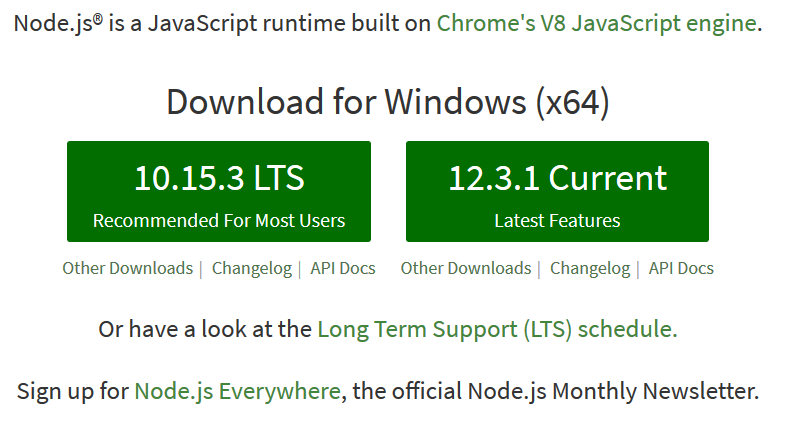
\includegraphics[width=0.6\textwidth]{./IoT/MicrosoftAzure/4-3-1_send_simulated_telemetry.png}
 \caption{Descarga de Node.js desde el sitio web oficial.}
 \label{downloadnode}

\end{figure}

Acorde a la documentación, también es necesario ejecutar el comando
\hyperref[eq:azurecli]{\ref{azurecli}}

\begin{equation}
 \label{eq:azurecli}
 az extension add --name azure-cli-iot-ext
\end{equation}

El cual agrega la extensión IoT de Azure para la CLI a la instancia de Cloud
Shell.

Por último, en caso de no contar con un dispositivo que conectar, siempre puede
emplearse lo proporcionado en 
\url{https://github.com/Azure-Samples/azure-iot-samples-node/archive/master.zip}

\subsubsection{Creación de un centro de IoT}

Dentro de Azure portal, cuyo acceso no merece mención debido a la experiencia
por parte del lector en este tema, se busca ``IoT Hub'' en la barra situada en
la parte superior del portal.

Una vez dentro de IoT Hub, se crea un nuevo recurso. La pantalla debería quedar
tal y como se puede ver en la captura
\hyperref[createresource]{\ref{createresource}}. Es necesario seleccionar el
grupo al cual pertenecerá el nuevo recurso y, en caso neceasrio, crear uno
nuevo. Por último, se selecciona un nombre para el IoT Hub (en este caso se ha
decidido que sea Hefesto, por ser el dios griego del fuego, la forja y los
artesanos; al ser el desarrollador que replique este proceso el que de forma y
esculpa el funcionamiento del dispositivo).

\begin{figure}[h!]
 \centering
 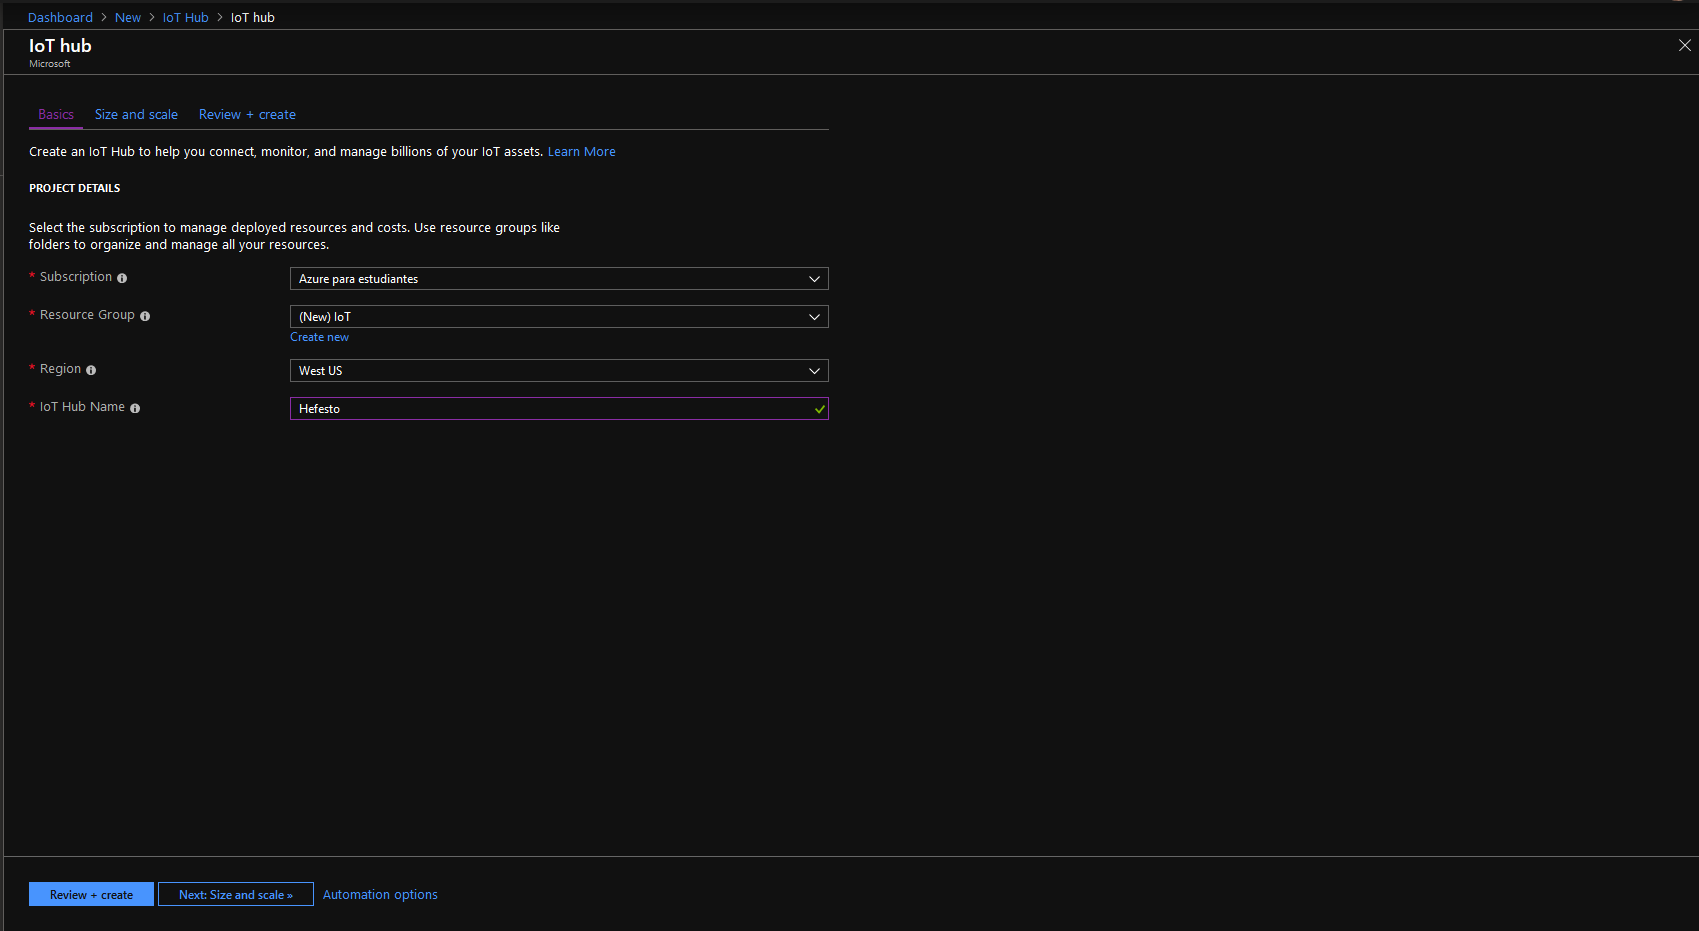
\includegraphics[width=0.7\textwidth]{./IoT/MicrosoftAzure/1-1_create_resource.png}
 \caption{Inicio del proceso de creación de recurso: asignación de Grupo y
 Nombre.}
 \label{createresource}
\end{figure}

Una vez finalizados los pasos de la explicación anterior, se pasa al siguiente
punto, definición del tamaño y la escala \hyperref[sizescale]{\ref{sizescale}}.
En esta página, tal y como su nombre indica, se seleccionarán el tamaño (número
de unidades) y la escala (de entre las que proporciona Microsoft Azure). De las
escala, cabe añadir que se encuentran los siguientes tipos:

\begin{easylist}[itemize]
  & Estándar (desde S1 hasta S3).
  & Básico (desde B1 hasta B3).
  & Gratuito. De este cabe decir que solo se emplea para pruebas y evaluaciones.
  Permite 500 dispositivos con el centro de IoT y hasta 8000 mensajes al día.
  Solo puede crearse una instacia \cite{azure_iot}.
\end{easylist}

\begin{figure}[h!]
 \centering
 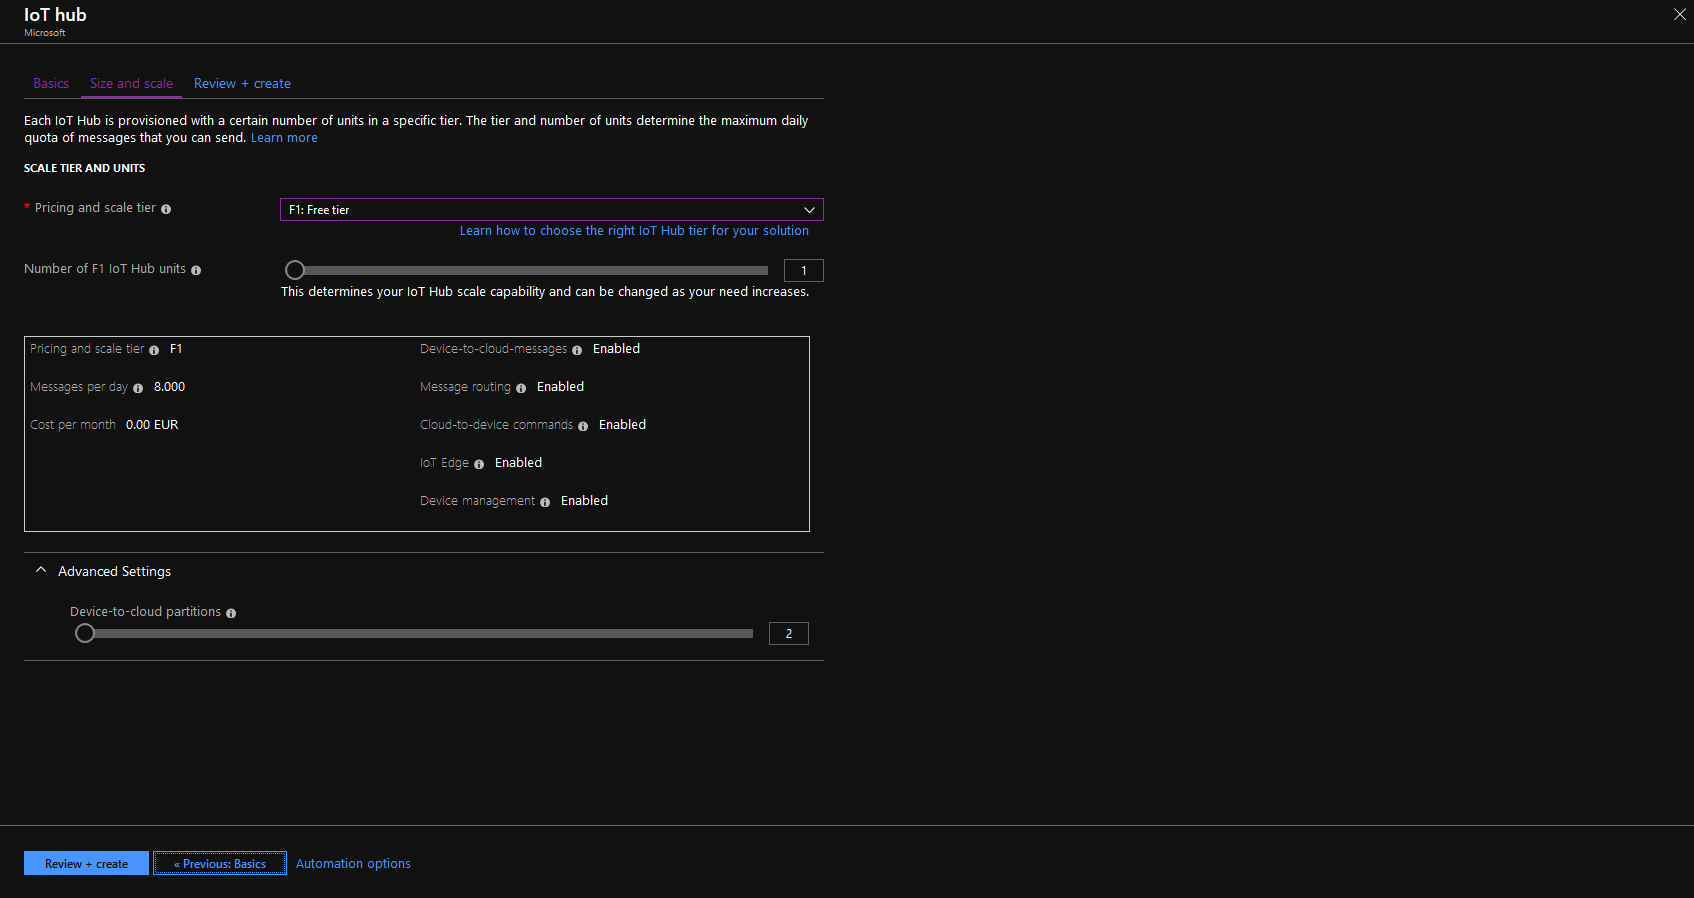
\includegraphics[width=0.7\textwidth]{./IoT/MicrosoftAzure/1-2_create_resource.png}
 \caption{Seleccionar tamaño y escalabilidad}
 \label{sizescale}
\end{figure}

Se puede pasar a revisar y crear la unidad IoT Hub \hyperref[review]{\ref{review}}.

\begin{figure}[h!]
 \centering
 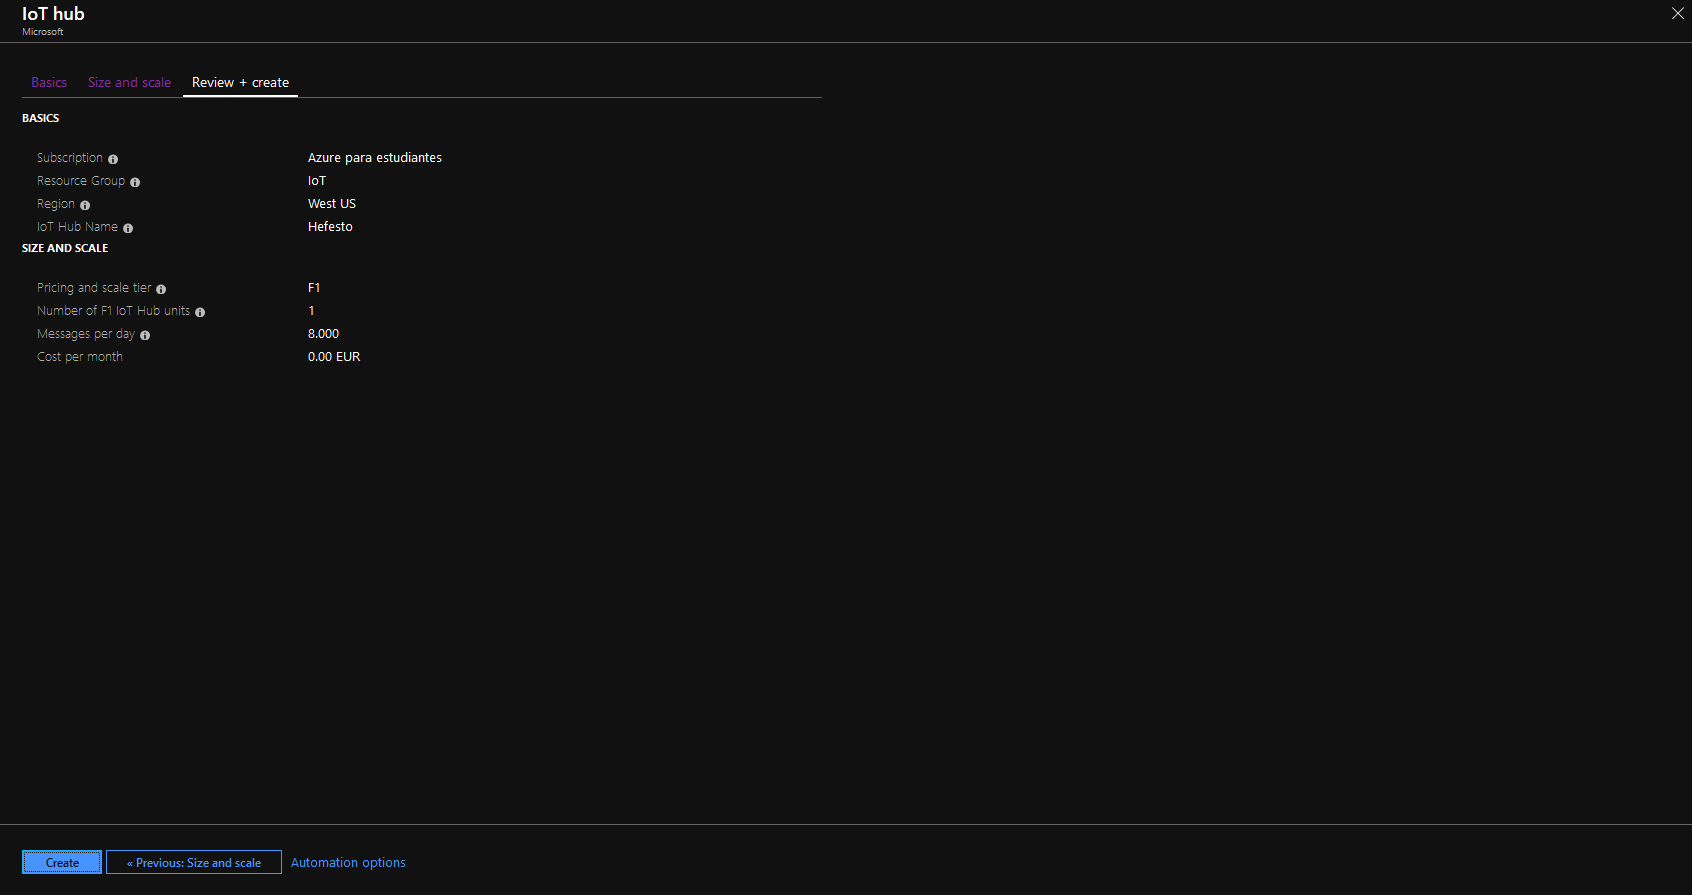
\includegraphics[width=0.7\textwidth]{./IoT/MicrosoftAzure/1-3_create_resource.png}
 \caption{Revisión y Creación.}
 \label{review}
\end{figure}

\subsubsection{Registrar Dispositivo}

Para registrar el dispositivo que se va a emplear, es necesario acceder a la
terminal de Azure. No se va a proporcionar ninguna explicación de como acceder a
la misma, debido a que el lector ya es consciente de como llegar hasta ella.

Primero, se debe empezar por crear la identidad del dispositivo 
\hyperref[register]{\ref{register}}, con la que será referido a partir de ahora 
mediante el comando:

\begin{equation}
 \label{deviceid}
 az iot hub device-identity create --hub-name YourIoTHubName --device-id 
 MyNodeDevice
\end{equation}

Dentro de \hyperref[deviceid]{\ref{deviceid}} se debe sustituir YourIoTHubName
por el nombre del Hub, que en este caso será Hefesto; y MyNodeDevice por el
nombre del dispositivo, se ha dejado tal cual por mera comodidad, al tener esta
práctica como objetivo aprender a usar las nociones básicas de las plataformas
Cloud.

Al ejecutar queda la siguiente traza \hyperref[register]{\ref{register}}:

\begin{figure}[h!]
 \centering
 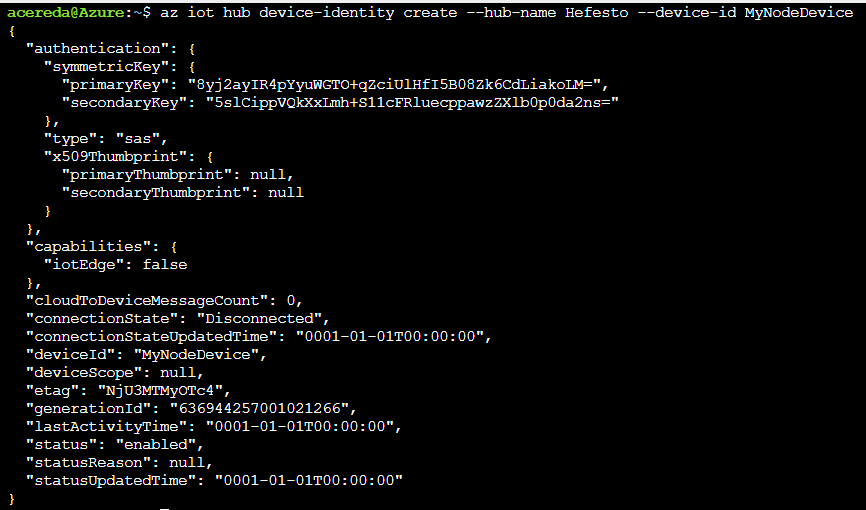
\includegraphics[width=0.8\textwidth]{./IoT/MicrosoftAzure/3-1_register_device.png}
 \caption{Registro del dispositivo.}
 \label{register}
\end{figure}

Acto seguido, se debe conseguir la cadena de conección perteneciente a al
dispositivo. Una vez más, se debe ejecutar en la consola un comando:

\begin{equation}
 \label{condevcommand}
 az iot hub device-identity show-connection-string --hub-name YourIoTHubName 
  --device-id MyNodeDevice --output table
\end{equation}

Una vez más, se sustituye YourIoTHubName por Hefesto, que es al que se quiere
hacer referencia. La cadena resultante de la ejecución del comando debe 
guardarse \hyperref[constring]{\ref{constring}} para, posteriormente, poder 
realizar la conexión con el disposito.

\begin{figure}[h!]
 \centering
 \includegraphics[width=0.7\textwidth]{./IoT/MicrosoftAzure/3.2_register_device.png}
 \caption{Conexión con el dispositivo.}
 \label{constring}
\end{figure}

Finalmente, se debe hacer de manera similar, pero en este caso con la cadena de
conexiónde servicio. Este último permite conectarse al IoT Hub y recuperar los
mensajes enviados por el dispositivo.

\begin{equation}
 \label{consercommand}
az iot hub show-connection-string --name YourIoTHubName --output table
\end{equation}

\subsubsection{Envío de datos de telemetría simulados}

Todo lo hecho anteriormente está muy bien y tal\ldtos, pero no es una
``aplicación real''. El dispositivo debería poder mandar datos al fin y al cabo.
Para ello se debe abrir una terminal local, e ir al directorio donde se ha
descargado, en este caso, el ejemplo del repositorio Git proporcionado
anteriormente en este documento. Se debe entrar al directorio
\textit{iot-hub/Quickstarts/simulated-device}
\hyperref[directory]{\ref{directory}}.

\begin{figure}[h!]
 \centering
 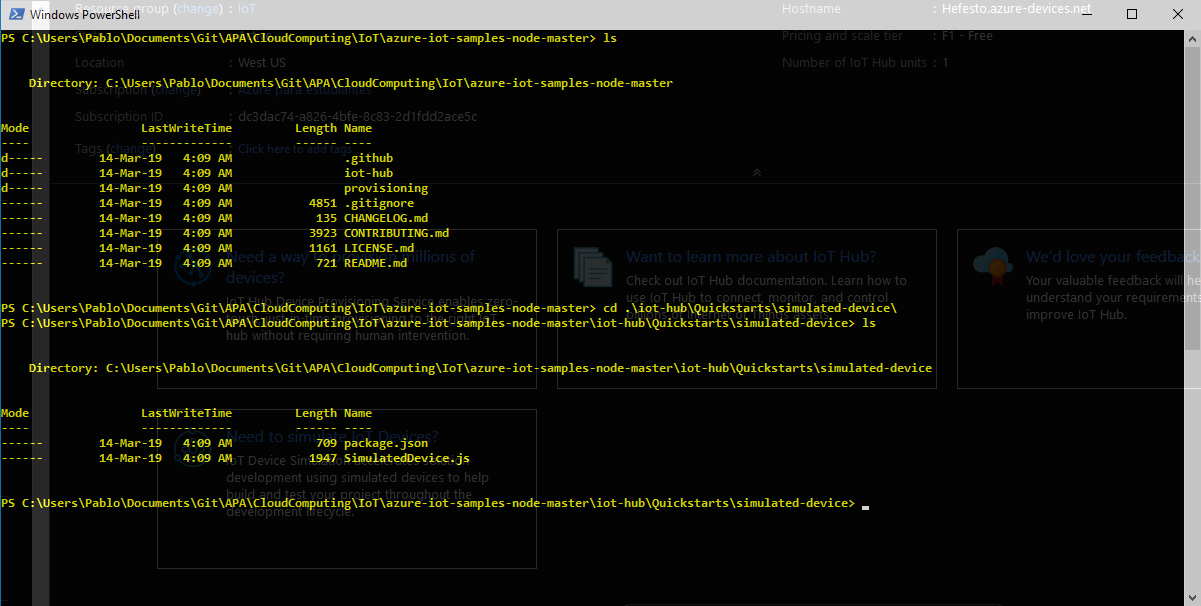
\includegraphics[width=0.8\textwidth]{./IoT/MicrosoftAzure/4-1_send_simulated_telemetry.png}
 \caption{Conexión con el dispositivo.}
 \label{directory}
\end{figure}

Debe sustituirse el contenido de \textit{connectionString}
\hyperref[directory]{\ref{directory}} a la salida obtenida en la ejecución de 
\hyperref[condevcommand]{\ref{condevcommand}} en el archivo SimulatedDevice.js.

\begin{figure}[h!]
 \centering
 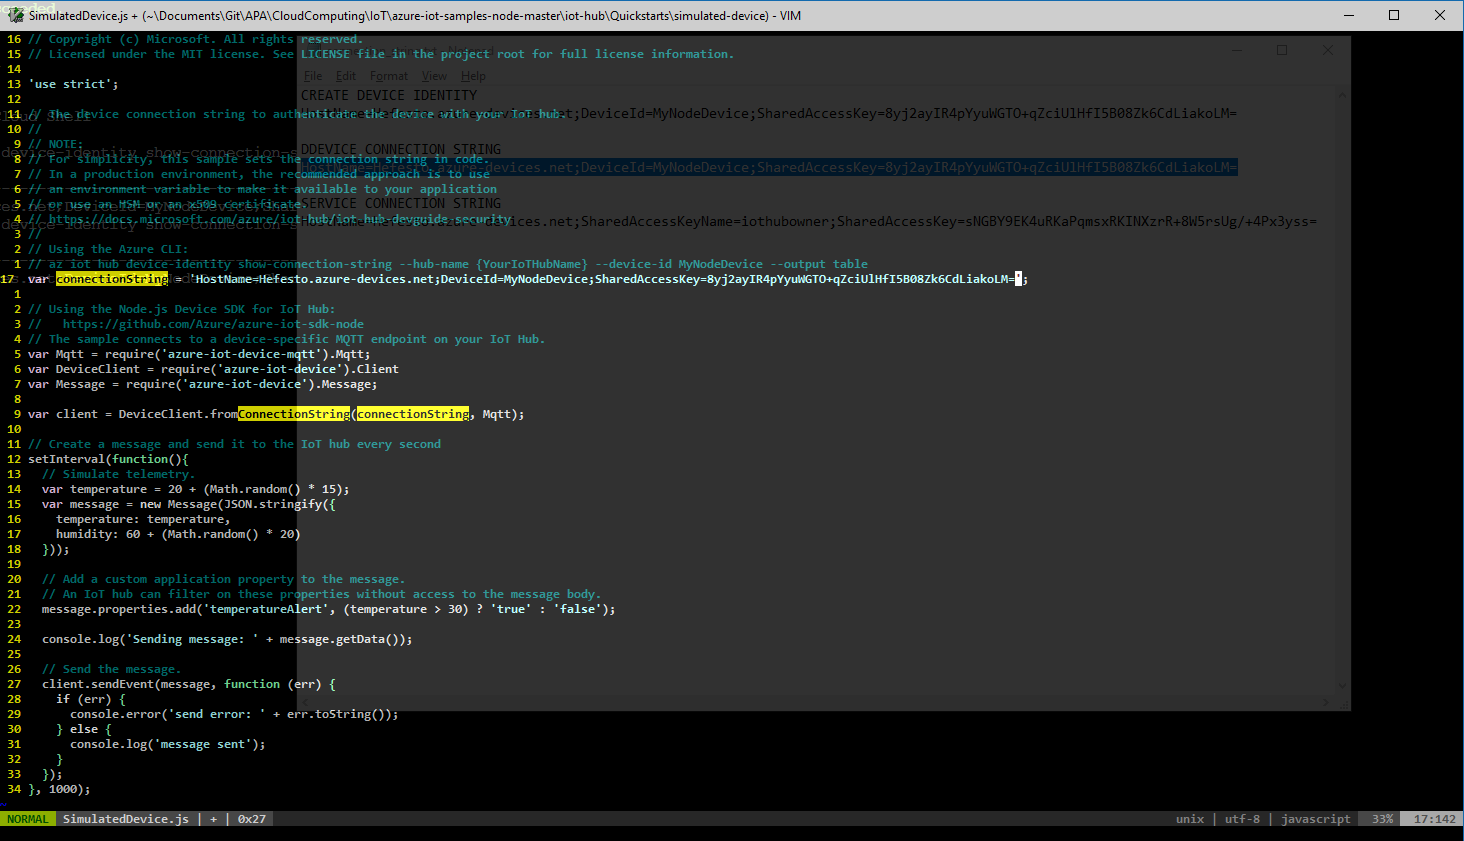
\includegraphics[width=\textwidth]{./IoT/MicrosoftAzure/4-2_send_simulated_telemetry.png}
 \caption{Cadena de conexión del dispositivo.}
 \label{codestring}
\end{figure}

Tras guardar el archivo, ya puede ejecutarse el código:

\begin{equation}
 \label{ejecdev1}
npm install
\end{equation}

\begin{equation}
 \label{ejecdev2}
node SimulatedDevice.js
\end{equation}

\begin{figure}[h!]
 \centering
 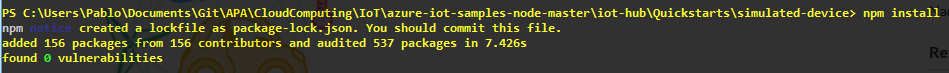
\includegraphics[width=0.7\textwidth]{./IoT/MicrosoftAzure/4-4_send_simulated_telemetry.png}
 \caption{Instalación de paquetes necesarios para la ejecución.}
 \label{npmdev}
\end{figure}

El resultado de la ejecución da el siguiente resultado
\hyperref[nodedev]{\ref{nodedev}}, que como se puede observar hace referencia a 
los mensajes enviados por el disposito.

\begin{figure}[h!]
 \centering
 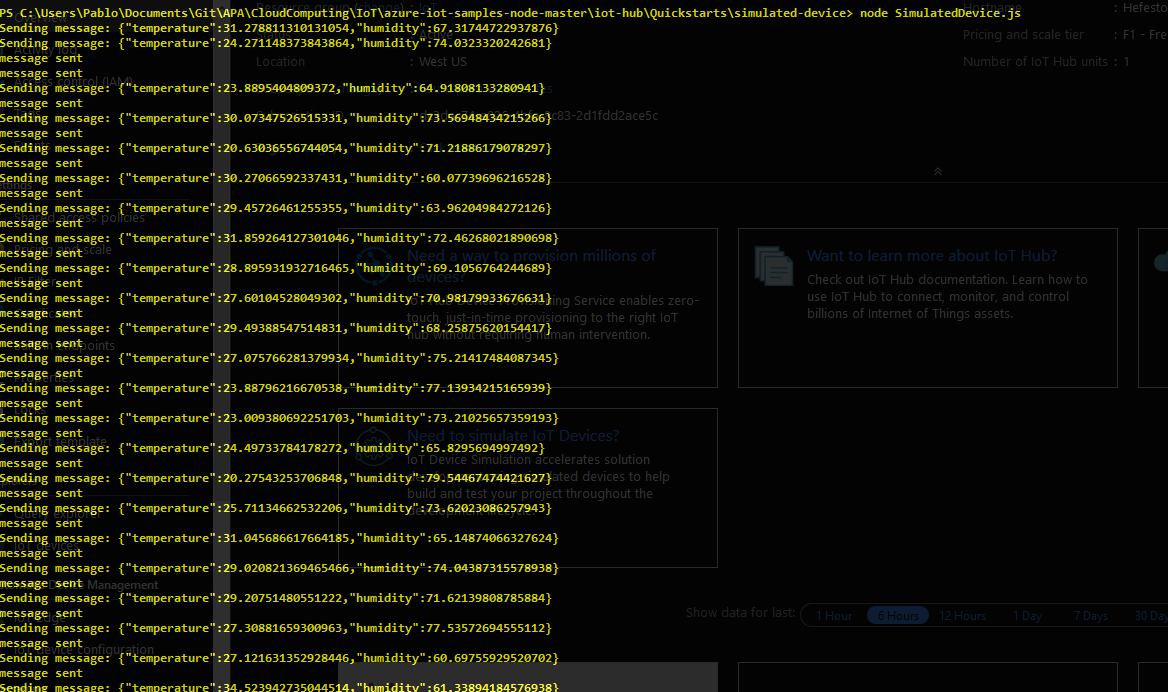
\includegraphics[width=\textwidth]{./IoT/MicrosoftAzure/4-5_send_simulated_telemetry.png}
 \caption{Conexión con el dispositivo.}
 \label{nodedev}
\end{figure}

\subsubsection{Lectura de los datos de telemetríá procedentes de su instancia de
IoT Hub}

Pero no solo hay que mandar datos, también hay que ser capaz de leerlos. En este
apartado se explica como crear un proceso que tome los datos del dispositivo,
desde IoT Hub, y los lea. Para ello hace falta otra instancia de la terminal
local. En este caso, en lugar de la ruta \textit{simulated-device}, se accede a
la ruta \textit{iot-hub/Quickstart/read-d2c-messages}
\hyperref[directoryreader]{\ref{directoryreader}}.

\begin{figure}[h!]
 \centering
 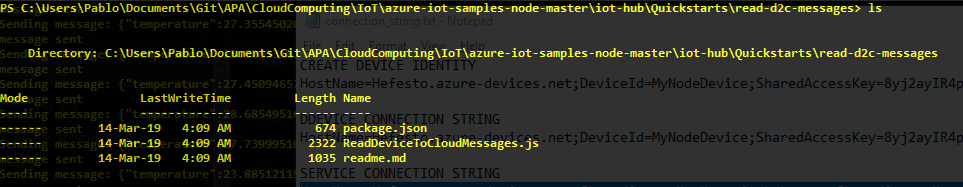
\includegraphics[width=0.7\textwidth]{./IoT/MicrosoftAzure/5-1_read_telemetry.png}
 \caption{Lectura de datos del dispositivo.}
 \label{directoryreader}
\end{figure}

Al igual que en el caso de la escritura de datos, en la lectura de datos es
necesario especificar en el fichero ReadDeviceToCloudMessages.js. En este caso
el contenido de \textit{connectionString} debe sustituirse
\hyperref[codestringser]{\ref{codestringser}} por lo obtenido en la cadena de 
conexión de servicio \hyperref[consercommand]{\ref{consercommand}}.

\begin{figure}[h!]
 \centering
 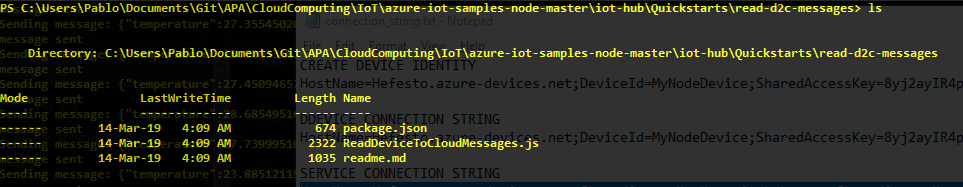
\includegraphics[width=0.6\textwidth]{./IoT/MicrosoftAzure/5-1_read_telemetry.png}
 \caption{Cadena de conexión a servicio.}
 \label{codestringser}
\end{figure}

Una vez más, debe ejecutarse \hyperref[ejecdev1]{\ref{ejecdev1}}, seguido de
\hyperref[ejecdev3]{\ref{ejecdev3}}.

\begin{equation}
 \label{ejecdev3}
node ReadDeviceToCloudMessages.js
\end{equation}

El resultado de la ejecución del comando anterior
(\hyperref[ejecdev3]{\ref{ejecdev3}}) puede observarse en la captura 

\begin{figure}[h!]
 \centering
 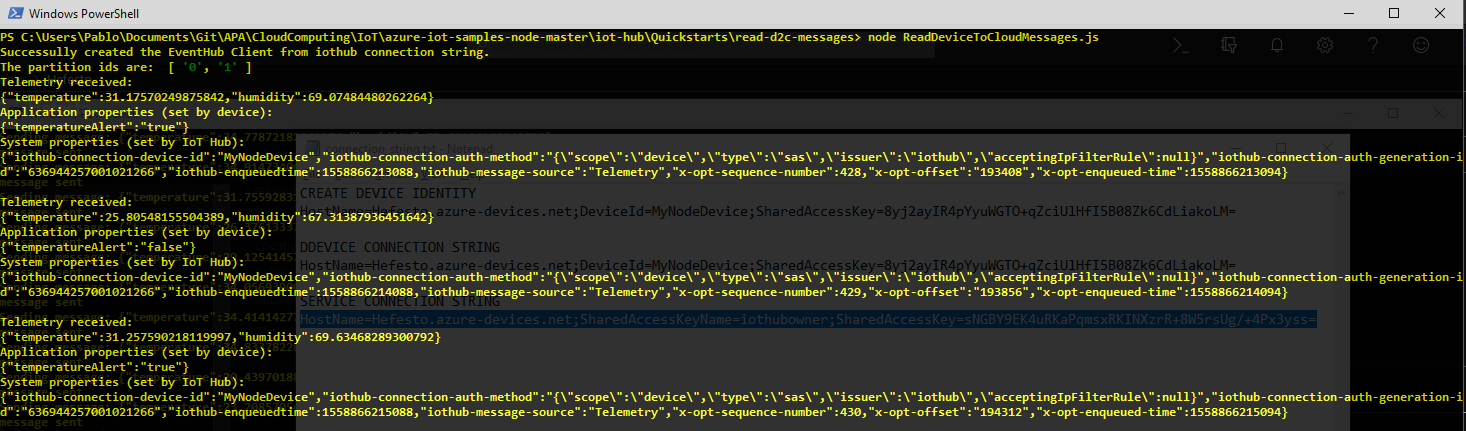
\includegraphics[width=0.9\textwidth]{./IoT/MicrosoftAzure/5-4_read_telemetry.png}
 \caption{Cadena de conexión a servicio.}
 \label{nodeser}
\end{figure}

\subsection*{Amazon Web Service}
% TODO: Poner que se va a hacer

\subsubsection{Crear la política de AWS IoT}

Para comenzar con el desarrollo, es necesario entrar crear una política que se
adapte al nuevo recurso. Para ello se debe primero entrar a  
\url{https://aws.amazon.com} e iniciar sesión. Una vez iniciada la sesión, en la
barra de navegación (zona superior, en azul oscuro), parte derecha, se debe
seleccionar la región de AWS en la que se van a crear los recursos (la
documentación recomienda \textit{Norte de Virgina}).

Para seguir con el proceso, se debe buscar por \textit{IoT Core} 

\begin{figure}[h!]
 \centering
 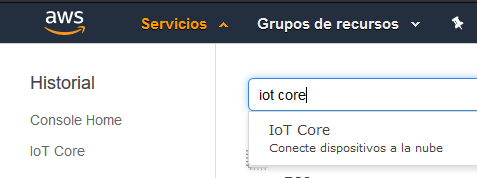
\includegraphics[width=0.7\textwidth]{./IoT/AWS/1-2_search_iot_core.png}
 \caption{Búsqueda de servicio IoT Core.}
 \label{search}
\end{figure}

Dentro de la página abierta tras clickar sobre \textit{IoT Core}, en el menú
contextual del marguen izquierdo se debe pulsar en la pestaña de políticas, 
dentro de Seguro \hyperref[policies]{\ref{policies}}.

\begin{figure}[h!]
 \centering
 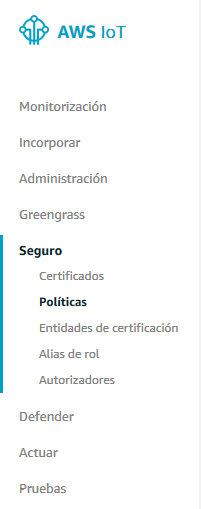
\includegraphics[width=0.7]{./IoT/AWS/1-3_politics.png}
 \caption{Selección de opción de Políticas.}
 \label{policies}
\end{figure}

Esto permite visualizar las posibles políticas existentes, y en caso de que no
exista una, crearla. En este caso, se parte de la terminal del desarrollador,
que en efecto carece de políticas preexistentes, así que se pulsa ``Crear''.

Dentro de la ventana, se debe proporcionar un nombre a la nueva política. En
este caso, y siguiendo el ejemplo encontrado, la política recibirá´el nombre de
\textbf{PlantWateringPolicy}. 

En las declaraciones que se encuetran debajo del nombre debe escribirse:

\begin{easylist}[itemize]
  & \textbf{Acción: } iot:*
  & \textbf{ARN de recurso: } Se debe sustituir el valor recomendado por *.
  & \textbf{Efecto: } Se debe elegir \textit{Permitir}
\end{easylist} 

Por último, se crea la política \hyperref[newpolicy]{\ref{newpolicy}}.

\begin{figure}[h!]
 \centering
 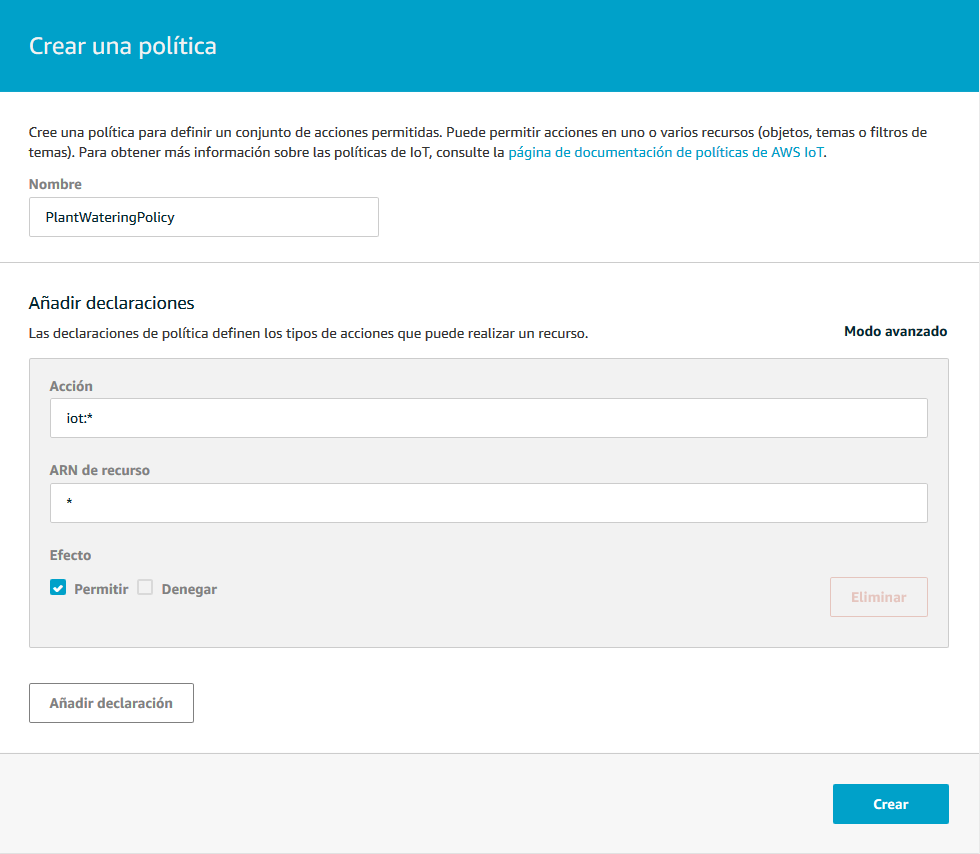
\includegraphics[width=0.7\textwidth]{./IoT/AWS/1-4_create_policy.png}
 \caption{Creación de una nueva política.}
 \label{newpolicy}
\end{figure}

\subsubsection{Crear el objeto}

A continuación se explica como construir un objeto para representar el
dispositivo que mande los mensajes dentro de la red IoT.

De vuelta a la consola de administración de AWS, es necesario buscar por
\textit{IoT Device Management} y seleccionarlo \hyperref[search2]{\ref{search2}}.

\begin{figure}[h!]
 \centering
 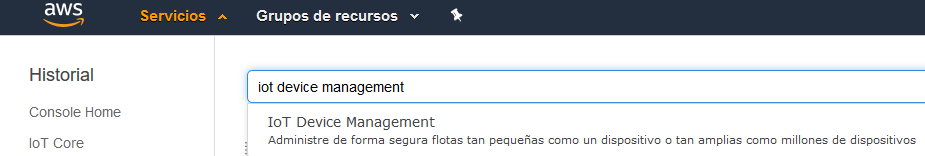
\includegraphics[width=0.7\textwidth]{./IoT/AWS/2-1_search.png}
 \caption{Búsqueda de servicio IoT Device Management.}
 \label{search2}
\end{figure}

Debería abrirse de manera predeterminada en Objetos, dentro de la sección de
Administración. En caso contrario, ir a esta sección del menú izquierdo.

Al igual que antes, en caso de que no exista un objeto, este se debe registrar
(``Registrar un objeto'').

De las opciones que se plantean (Registrar un solo objeto de AWS Iot o Registrar
por lotes muchos objetos de AWS IoT), se debe elegir la primera opción: ``Crear
un solo objeto''.

A continuación se debe rellenar la información del desplegable. 

\begin{easylist}[itemize]
  & Darle un nombre al dispositivo que se va a añadir \hyperref[name]{name}. En 
  este caso, va a llamarse Hefestus, por las mismas razones que recibió ese 
  nombre en el proceso de la plataforma Microsoft Azure.
  & El resto de elementos deben mantenerse de manera predeterminada, con us
  valores sin cambiar.
\end{easylist}

\begin{figure}[h!]
 \centering
 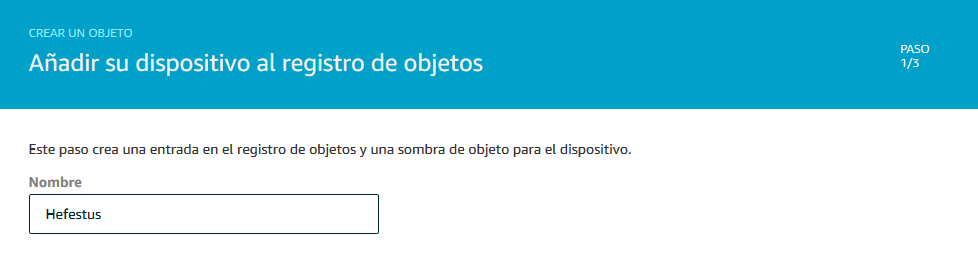
\includegraphics[width=0.7\textwidth]{./IoT/AWS/2-2_name.png}
 \caption{Creación de objeto, nombramiento.}
 \label{name}
\end{figure}

Posteriormente, debe pulsarse ``Siguiente'', accediéndose a la pestaña de
certificados del objeto. De entre las opción presentadas, se debe elegir la
primera de ellas: Creación de un certificado con un clic (recomendado); pulsar
el botón ``Crear un certificado''.

Ahora es turno de descargar ``Un certificado para este objeto'', ``Una clave
pública'', ``Una clave privada'' además de ``Una entidad de certificación raíz
para AWS IoT''; tal y como se muestra en la captura
\hyperref[certificate]{\ref{certificate}}.

El último de los anteriormente mencionados, permite obtener la clave RSA de 2048
bits.

\begin{figure}[h!]
 \centering
 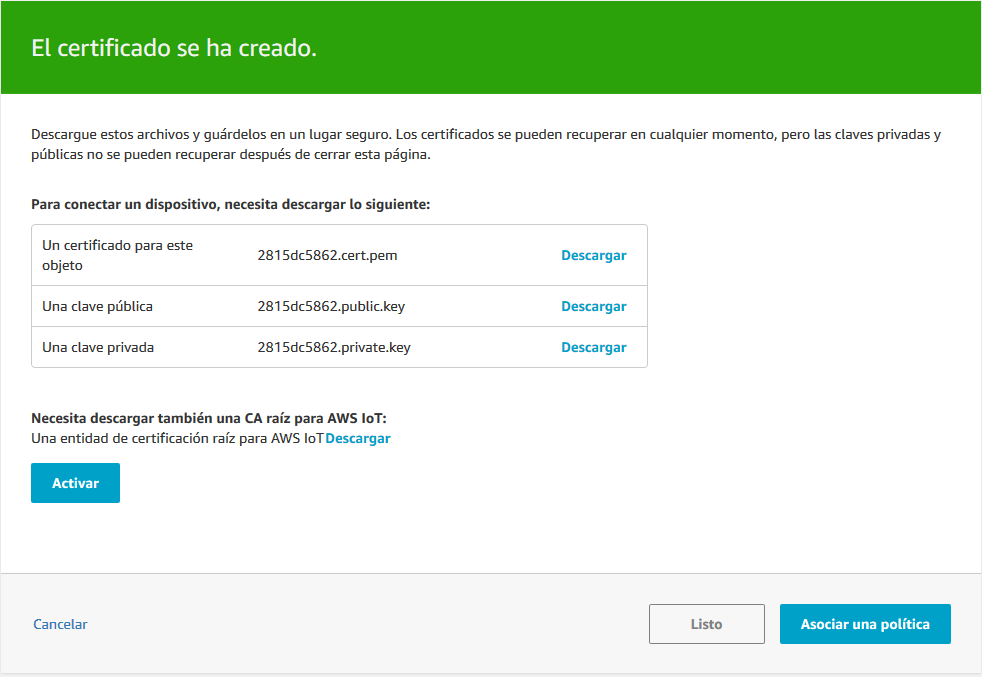
\includegraphics[width=0.7\textwidth]{./IoT/AWS/2-3_certificate.png}
 \caption{Creación y descarga de certificados.}
 \label{certificate}
\end{figure}

Como punto final, pulsar sobre ``Activar''.

Acto seguido, se debe ``Asociar una política'', donde se puede añadir una
política al objeto ya creado.  En este caso, la política asociada será la que se
ha creado con anterioridad: \textit{PlantWateringPolicy} y se ``Registra
objeto'' \hyperref[assignmentpolicy]{\ref{assignmentpolicy}}

\begin{figure}[h!]
 \centering
 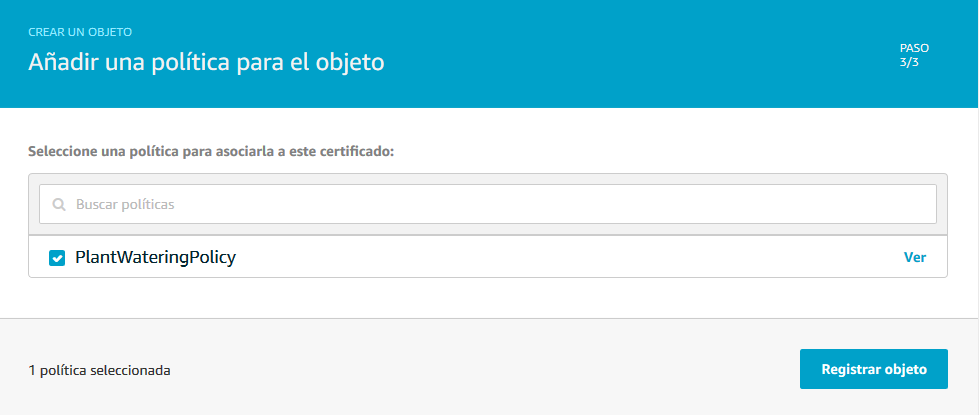
\includegraphics[width=0.7\textwidth]{./IoT/AWS/2-4_policy.png}
 \caption{Asignación de política.}
 \label{assignmentpolicy}
\end{figure}

\subsubsection{Enviar y recibir datos de prueba para el objeto}

En esta parte del desarrollo, en necesario entrar en el Objeto creado y pulsar
``Interactuar'' en la sección izquierda.

Como se puede observar, se muetras información sobre HTTPS y MQTT. Del segundo,
se debe guardar la información proveniente de:

\begin{easylist}[itemize]
  & Actualizar a esta sobre de dispositivo.
  & Obtener esta sobra de dispositivo.
  & Aceptar esta sobrea de dispositivo.
\end{easylist}

Volviendo a la vista de objetos (la ventana anterior), ir a la pestaña de
Pruebas.

Dentro de esta sección, se van a usar las direcciones guardadas anteriormente.
En la parte superior, donde pone ``Tema de suscripción'' se deben pegar una a
una las rutas copiadas anteriormente \hyperref[suscription]{\ref{suscription}}.

\begin{figure}[h!]
 \centering
 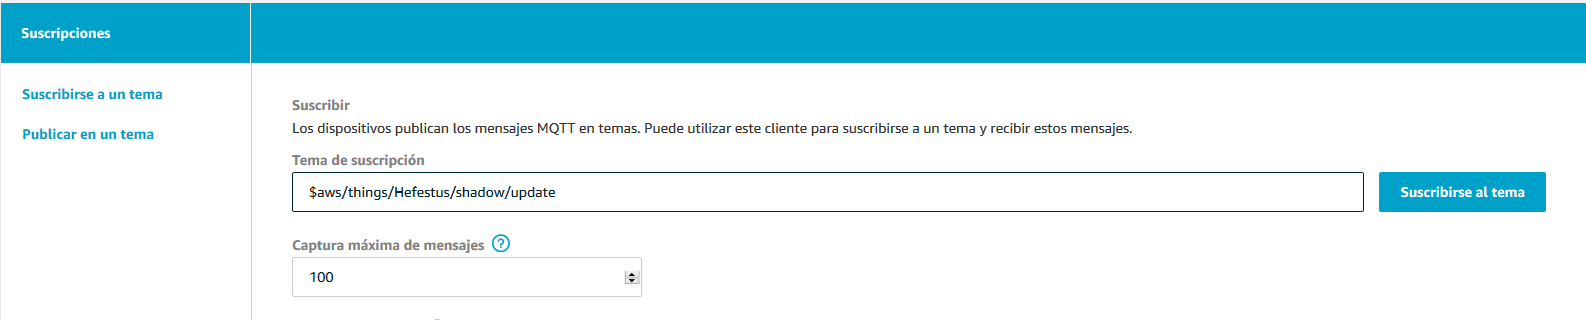
\includegraphics[width=0.7\textwidth]{./IoT/AWS/3-1_suscription.png}
 \caption{Suscripción a tema.}
 \label{suscription}
\end{figure}

Para comprobar que el proceso se ha desarrollado de manera correcta, se debe
realizar una inserción de valores dentro de alguno de los temas a los que está
suscrito el cliente de MQTT. 

Se ha decidido usar el tema de actualización (update) debido a que es el mismo
usado en el ejemplo seguido para llevar a cabo esta práctica
\hyperref[insertion]{\ref{insertion}}.

\begin{figure}[h!]
 \centering
 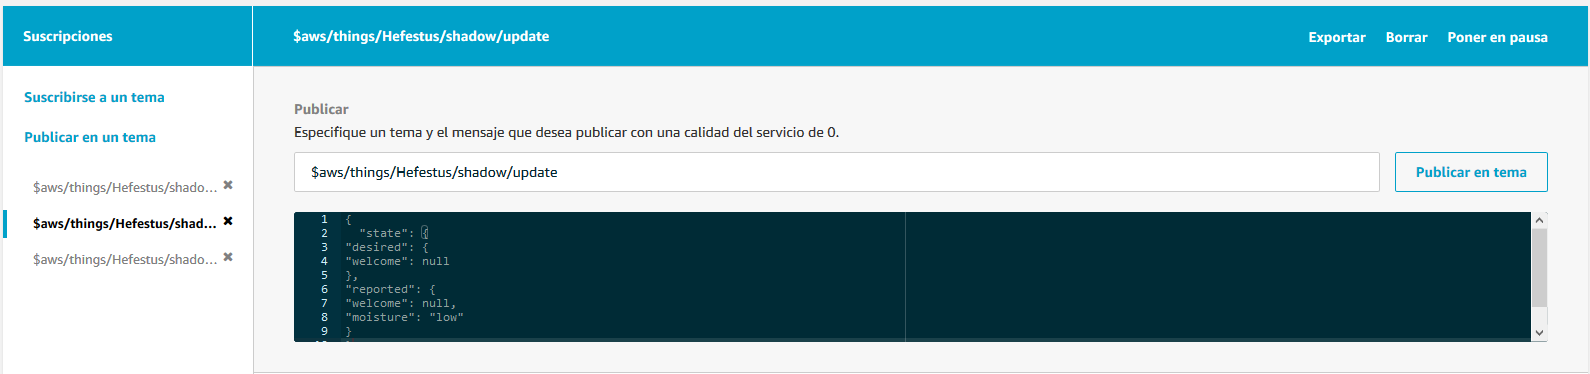
\includegraphics[width=0.7\textwidth]{./IoT/AWS/3-2_insertion.png}
 \caption{Inserción de datos dentro de un tema.}
 \label{insertion}
\end{figure}

Esta sustitución del contenido de ``update'' le da un valor diferente al de
bienvenida, lo que puede emplearse para simular el funcionamiento del sensor.
Tras publicar dicho tema, estos pueden ser obtenidos si se accede al tema
``get''. 

Dentro del mismo se debe eliminar el contenido del tema, dejando solamente los
corchetes ({}). Posteriormente tan solo es necesario publicar el tema.

La carencia de contenido dentro de ``get'' provoca que ``accepted'' reciba los
datos provenientes de ``update'' tras cada publicación de un nuevo tema
\hyperref[accepted]{\ref{accepted}}.

\begin{figure}[h!]
 \centering
 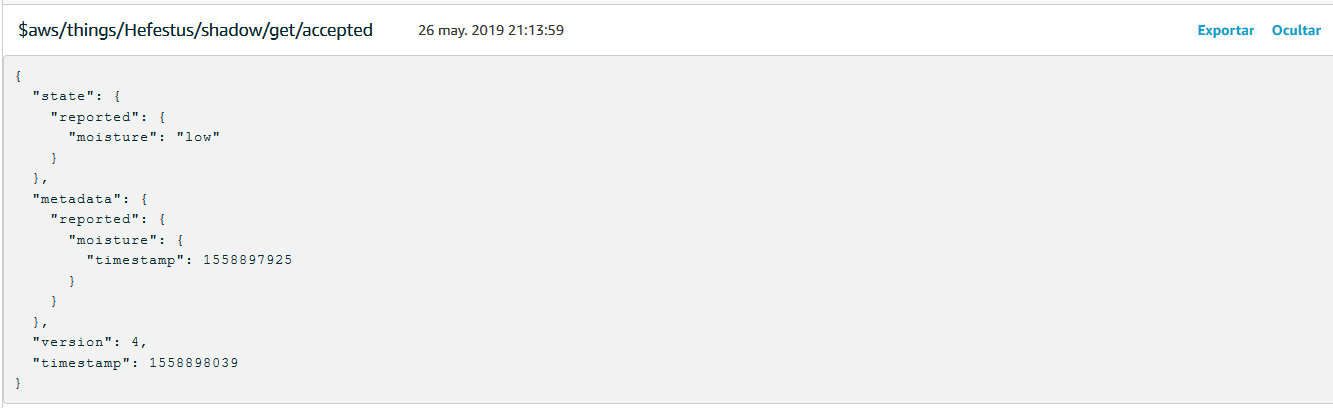
\includegraphics[width=0.7\textwidth]{./IoT/AWS/3-3_accepted.png}
 \caption{Datos recibidos tras una publicación de tema.}
 \label{accepted}
\end{figure}

Con el objetivo de responder a cada evento publicado, también se cambia el
contido del mensaje de ``update''. En este caso no se va a proporcionar una
captura, parece algo innecesario cuando lo único que se ha hecho es cambiar el
contenido del mensaje.

Mediante sustituiciones y publicaciones de los diferentes componentes de
publicación del cliente se puede mandar y recibir mensajes. El proceso sería el
siguiente:

\begin{easylist}[enumerate]
  & Desde update, generar el mensaje deseado y publicarlo.
  & Reducir el mensaje contenido en get a unos meros corchetes ({}) y publicar
  el mensaje.
  & Finalmente, accepted recuperará el mensaje enviado por update.
\end{easylist}

\subsection{Comparativa}

Para comparar ambas plataformas, se inverstigarán las características respectica
a cada una de ellas referentes al apartado IoT (con la información obtenida en
\cite{compiot}),y posteriormente se procederá a evaluar la experiencia que se ha
tenido con cada plataforma.

A rasgos generales, puede verse que ambas plataformas son muy similares y
ofrecen servicios realmente parecidos. Esto es muy fácilmente entendible, debido
a que al ser ambas dos de las grandes competidoras por los servicios Cloud, ``se
copian entre ellas''; tiene todo el sentido si se para a pensar en ello, si
Azure saca una característica para IoT que AWS no tiene incluido en su
plataforma, este acabará por desarrollarlo para ponerse a la par con su
competidor.

A nivel más técnico, Azure puede parecer más apetecible a grandes empresas por
su control nativo de AD (Active Directory) lo que, en combinación con otras
metodologías, facilita la integración con aplicaciones más antiguas existentes
dentro de la compañía.

En cuanto a nivel de comunicación, ambos sistemas aceptan los mismos protocolos,
aunque con Azure no es tan sencillo usar HTTP (por motivos de securización de
infraestructuras). HTTP necesita de IoT Hub y una puerto personalizado para
poder operar dentro de Azure.

De nuevo, no pueden encontrarse apenas diferencias entre ambas plataformas;
aunque en esta ocasión se hable de lenguajes de programación, o de tratamiento 
de los sitemas IoT (Hadoop, Spark y R), aceptados dentro de las mismas.

Los sistemas de monitorización empleados por ambas plataformas son prácticamente
idénticos: almacenamiento backend, se puede comprobar el estado de los
diferentes componentes de la red IoT\ldots

En comunicación ambas plataformas ofrecen el mismo servicio y de manera muy
similar, la única diferencia es que AWS ofrece un motor de reglas. Por otro
lado, Azure emplea dos \textit{endpoints} que se emplean para recibir y mandar
información.

En seguridad ambos emplean TLS (Transport Layer Security) para su comunicación.

Ambas plataformas ofrecen servicios similares, pero Azure tiene una mayor
cantidad de servicios que soportan IoT, pero por otro lado AWS subre esas mismas
necesidades con una menor cantidad de servicios.

Además, Azure es más barato que Amazon. Ambos proveedores ofrencen niveles
gratuitos para la prueba y testeo de IoT.

A nivel de experiencia personal, Azure es una plataforma más cómoda de usar. AWS
cada hora hace caducar la sesión, con lo cual hace falta volver a iniciarla en
caso de que se haya superado este límite (algo extremadamente tedioso cuando
estás haciendo algo en la plataforma como escribir documentos, como esta
práctica, mientras se desarrollan los diferentes módulos IoT). Además, la
interfaz de Azure resulta más intuitiva, teniendo todas las funcionadidades a
``mano'' y sin necesidad de empezar a salir y entrar de la plataforma, buscar
fuera de internet.

Por otro lado, la documentación de Azure está muy a mano, y con explicaciones
concisas y detalladas (algo extraño en Windows a mi parecer); con AWS sin
embargo es muy complicado encontrar documentación, y en caso de hacer es un PDF
de 1000 páginas (como ha ocurrido en esta ocasión) en lugar de documentación en
su propia página, no como Azure, lo que acaba complicando mucho la navegación y
búsqueda de información a lo largo de la amplia documentación.

Azure además parece otorgar un mayor control a bajo nivel, al contar con
terminales (bash/Powershell); característica que no se ha encontrado en AWS.

Al parecer del desarrollador de este apartado, Azure es una apuesta más segura
que AWS; por su documentación, facilidad de uso\ldtos Así que en caso de tener
que emplear una de ellas en el futuro, sería Azure.

\section*{Bibliografía}

\printbibliography

\end{document}

